\documentclass{article}
\usepackage[utf8]{inputenc}
\usepackage{geometry}
\usepackage{graphicx}
\usepackage{wrapfig}
\usepackage{subfig}
\usepackage{subfigure}
\usepackage{amsmath}
\usepackage{amsfonts}
\usepackage{amsthm}
\usepackage[most]{tcolorbox}
\usepackage{fancybox}
\usepackage{verbatim}
\usepackage{array}
\usepackage{latexsym}
\usepackage{alltt}
\usepackage{hyperref}
\usepackage{textcomp}
\usepackage{color}
\usepackage{float}
\usepackage{pdfpages}
\usepackage{algorithm}
\usepackage[noend]{algpseudocode}
\usepackage{multicol}


\geometry
{
 a4paper,
 left=15mm,
 top=15mm,
}

\newtcolorbox{mybox}[3][]
{
  colframe = #2!25,
  colback  = #2!10,
  coltitle = #2!20!black,  
  title    = {#3},
  #1,
}

\renewcommand\qedsymbol{$\triangle$}

\newenvironment{example}{\begin{mybox}{green}{\textbf{Example}}}{\end{mybox}}
\newenvironment{definition}[1]{\begin{mybox}{blue}{\textbf{Definition #1}}}{\end{mybox}}
\newenvironment{theorem}[1]{\begin{mybox}{red}{\textbf{Theorem #1}}}{\end{mybox}}

\title{CENG223 - Chapter 11: Trees}
\author{Burak Metehan Tunçel}
\date{January 2022}

\begin{document}

\maketitle

\section{Introduction to Trees}

In this chapter, we will focus on a particular type of graph called a \textbf{tree}, so named because such graphs resemble trees. For example, family trees are graphs that represent genealogical charts. Family trees use vertices to represent the members of a family and edges to represent parent–child relationships.

\begin{mybox}{blue}{\textbf{Definition 1}}
A \textbf{\textit{tree}} is a connected undirected graph with no simple circuits.
\end{mybox}

Because a tree cannot have a simple circuit, a tree cannot contain multiple edges or loops. Therefore, \textit{any tree must be a simple graph}.

\begin{figure}[h!]
    \centering
    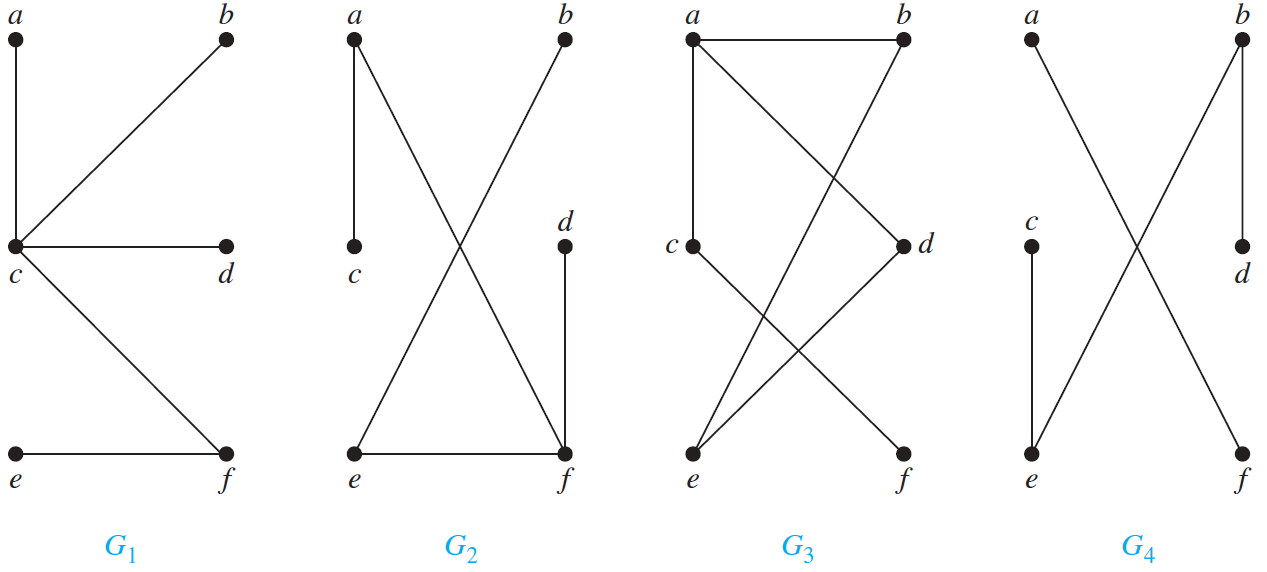
\includegraphics[width=.5\textwidth]{img/ch11-figure2.png}
    \caption{Examples of trees and graphs that are not trees}
    \label{fig:my_label}
\end{figure}
\begin{mybox}{green}{\textbf{Example}}
Which of the graphs shown in Figure 1 are trees?\\
\textbf{Solution:} $G_1$ and $G_2$ are trees, because both are connected graphs with no simple circuits. $G_3$ is not a tree because $e,\ b,\ a,\ d,\ e$ is a simple circuit in this graph. Finally, $G_4$ is not a tree because it is not connected.
\end{mybox}



\begin{wrapfigure}{r}{.5\textwidth}
    \centering
    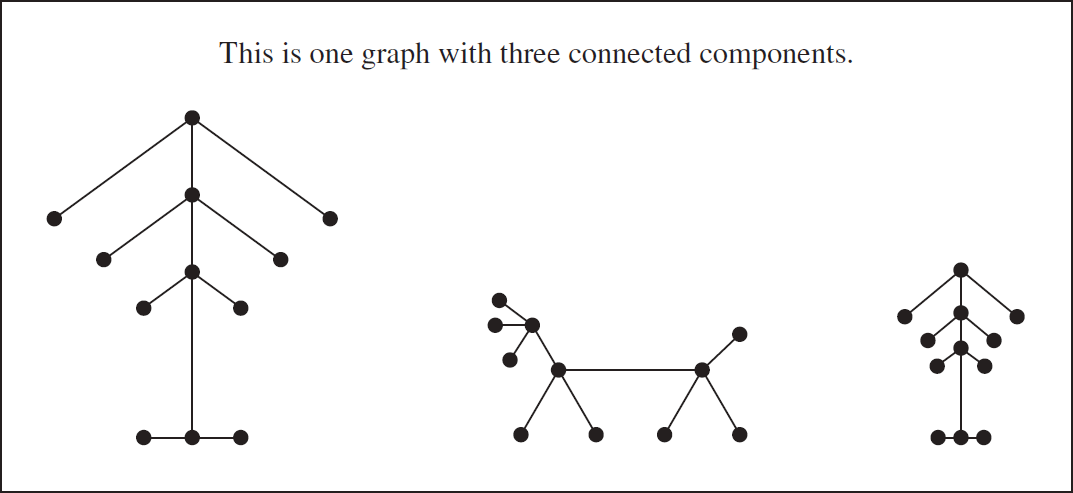
\includegraphics[width=.48\textwidth]{img/ch11-figure3.png}
    \caption{Example of a forest}
    \label{fig:my_label}
\end{wrapfigure}

\textit{Any connected graph that contains no simple circuits is a tree}. What about graphs containing no simple circuits that are not necessarily connected? These graphs are called \textbf{forests} and have the property that each of their connected components is a tree. Figure 2 displays a forest. Note that the graph $G_4$ in Figure 1 is also a forest. The graph in Figure 2 is a forest of three trees, while $G_4$ in Figure 1 is a forest of two trees.

Trees are often defined as undirected graphs with the property that there is a unique simple path between every pair of vertices. Theorem 1 shows that this alternative definition is equivalent to our definition.

\begin{mybox}{red}{\textbf{Theorem 1}}
An undirected graph is a tree if and only if there is a unique simple path between any two of its vertices.
\end{mybox}

\subsection{Rooted Trees}

In many applications of trees, a particular vertex of a tree is designated as the \textbf{root}. Once we specify a root, we can assign a direction to each edge as follows. Because there is a unique path from the root to each vertex of the graph (by Theorem 1), we direct each edge away from the root. Thus, a tree together with its root produces a directed graph called a \textbf{rooted tree}.

\begin{mybox}{blue}{\textbf{Definition 2}}
A \textit{\textbf{rooted tree}} is a tree in which one vertex has been designated as the root and every edge is directed away from the root.
\end{mybox}

Figure 3 displays the rooted trees formed by designating $a$ to be the root and $c$ to be the root, respectively, in the tree $T$.We usually draw a rooted tree with its root at the top of the graph. The arrows indicating the directions of the edges in a rooted tree can be omitted, because the choice of root determines the directions of the edges.

\begin{figure}[h!]
    \centering
    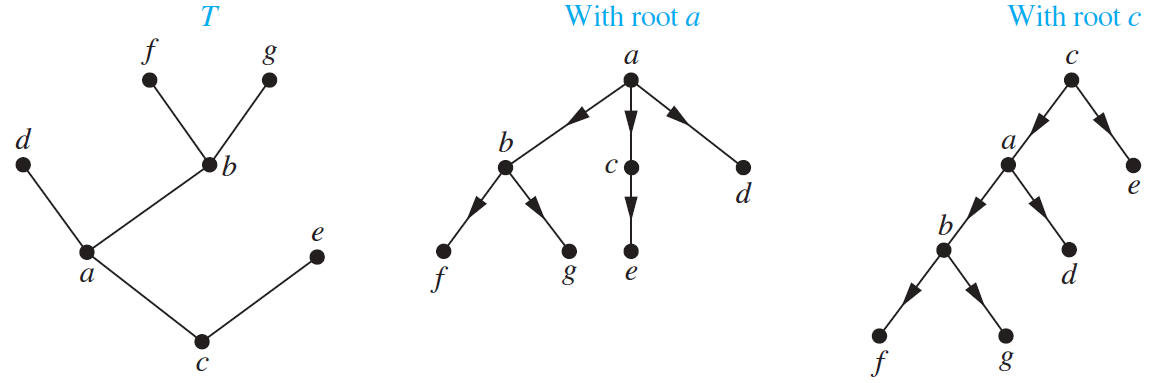
\includegraphics[width=.6\textwidth]{img/ch11-figure4.png}
    \caption{A tree and rooted trees formed by designating two different roots}
    \label{fig:my_label}
\end{figure}

The terminology for trees has botanical and genealogical origins. Suppose that $T$ is a rooted tree. If $v$ is a vertex in $T$ other than the root, the \textbf{parent} of $v$ is the unique vertex $u$ such that there is a directed edge from $u$ to $v$ . When $u$ is the parent of $v$, $v$ is called a \textbf{child} of $u$. Vertices with the same parent are called \textbf{siblings}. The \textbf{ancestors} of a vertex other than the root are the vertices in the path from the root to this vertex, excluding the vertex itself and including the root. The \textbf{descendants} of a vertex $v$ are those vertices that have $v$ as an ancestor. A vertex of a rooted tree is called a \textbf{leaf} if it has no children. Vertices that have children are called \textbf{internal vertices}. The root is an internal vertex unless it is the only vertex in the graph, in which case it is a leaf.

If $a$ is a vertex in a tree, the \textbf{subtree} with $a$ as its root is the subgraph of the tree consisting of $a$ and its descendants and all edges incident to these descendants.

\begin{mybox}{blue}{\textbf{Definition 3}}
A rooted tree is called an $m-ary$ tree if every internal vertex has no more than $m$ children. The tree is called a \textit{full} $m-ary$ tree if every internal vertex has exactly $m$ children. An $m$-ary
tree with $m = 2$ is called a \textit{binary tree}.
\end{mybox}

\subsubsection{Ordered Rooted Trees}

An \textbf{ordered rooted tree} is a rooted tree where the children of each internal vertex are ordered. Ordered rooted trees are drawn so that the children of each internal vertex are shown in order from left to right. Note that a representation of a rooted tree in the conventional way determines an ordering for its edges. We will use such orderings of edges in drawings without explicitly mentioning that we are considering a rooted tree to be ordered.

\newpage In an ordered binary tree (usually called just a \textbf{binary tree}), if an internal vertex has two children, the first child is called the \textbf{left child} and the second child is called the \textbf{right child}. The tree rooted at the left child of a vertex is called the \textbf{left subtree} of this vertex, and the tree rooted at the right child of a vertex is called the \textbf{right subtree} of the vertex.

Just as in the case of graphs, there is no standard terminology used to describe trees, rooted trees, ordered rooted trees, and binary trees. This nonstandard terminology occurs because trees are used extensively throughout computer science, which is a relatively young field.

\subsection{Trees as Models}

\textit{(Since this part consists of examples, it is better idea to read this part from the text book.)}

\subsection{Properties of Trees}

\begin{mybox}{red}{\textbf{Theorem 2}}
A tree with $n$ vertices has $n - 1$ edges.
\end{mybox}

Recall that a tree is a connected undirected graph with no simple circuits. So, when $G$ is an undirected graph with $n$ vertices, Theorem 2 tells us that the two conditions $(i)$ $G$ is connected and $(ii)$ $G$ has no simple circuits, imply $(iii)$ $G$ has $n - 1$ edges. Also, when $(i)$ and $(iii)$ hold, then $(ii)$ must also hold, and when $(ii)$ and $(iii)$ hold, $(i)$ must also hold. That is, if $G$ is connected and $G$ has $n - 1$ edges, then $G$ has no simple circuits, so that $G$ is a tree, and if $G$ has no simple circuits and $G$ has $n - 1$ edges, then $G$ is connected, and so is a tree. Consequently, when two of $(i)$, $(ii)$, and $(iii)$ hold, the third condition must also hold, and $G$ must be a tree.

\subsubsection{Counting Vertices In Full $m$-ary Trees}

The number of vertices in a full $m$-ary tree with a specified number of internal vertices is determined, as Theorem 3 shows. As in Theorem 2, we will use $n$ to denote the number of vertices in a tree.

\begin{mybox}{red}{\textbf{Theorem 3}}
A full $m$-ary tree with $i$ internal vertices contains $n = mi + 1$ vertices.
\end{mybox}

\begin{proof}
Every vertex, except the root, is the child of an internal vertex. Because each of the $i$ internal vertices has $m$ children, there are mi vertices in the tree other than the root. Therefore, the tree contains $n = mi + 1$ vertices.
\end{proof}


Suppose that $T$ is a full $m$-ary tree.
\begin{itemize}
    \item $n$ is the number of vertices
    \item $i$ is the number of internal vertices
    \item $l$ is number of leaves
\end{itemize}
in this tree. Once one of $n$, $i$, and $l$ is known, the other two quantities are determined. Theorem 4 explains how to find the other two quantities from the one that is known.

\begin{mybox}{red}{\textbf{Theorem 4}}
A full $m$-ary tree with
\begin{itemize}
    \item $n$ vertices has $i$ = $(n - 1)/m$ internal vertices and $l = [(m - 1)n + 1]/m$ leaves,
    \item $i$ internal vertices has $n = mi + 1$ vertices and $l = (m - 1)i + 1$ leaves,
    \item $l$ leaves has $n = (ml - 1)/(m - 1)$ vertices and $i = (l - 1)/(m - 1)$ internal vertices.
\end{itemize}
\end{mybox}

\subsubsection{Balanced $m$-ary Trees}

It is often desirable to use rooted trees that are “balanced” so that the subtrees at each vertex contain paths of approximately the same length. Some definitions will make this concept clear. The level of a vertex $v$ in a rooted tree is the length of the unique path from the root to this vertex. The level of the root is defined to be zero. The \textbf{height} of  rooted tree is the maximum of the levels of vertices. In other words, the height of a rooted tree is the length of the longest path from the root to any vertex.

A rooted $m$-ary tree of height $h$ is balanced if all leaves are at levels $h$ or $h - 1$.

\subsubsection{A Bound For The Number Of Leaves In An $m$-ary Tree}

It is often useful to have an upper bound for the number of leaves in an $m$-ary tree. Theorem 5 provides such a bound in terms of the height of the $m$-ary tree.

\begin{mybox}{red}{\textbf{Theorem 5}}
There are at most $m^h$ leaves in an $m$-ary tree of height $h$.
\end{mybox}

\begin{mybox}{purple}{\textbf{Corollary 1}}
If an $m$-ary tree of height $h$ has $l$ leaves, then $h \geq \lceil \log_m l \rceil$. If the $m$-ary tree is full and balanced, then $h = \lceil \log_m l \rceil$. (We are using the ceiling function here. Recall that $\lceil x \rceil$ is the smallest integer greater than or equal to $x$.)
\end{mybox}


\section{Applications of Trees}

\textit{(It is better idea to read this part from the text book)}.

%\subsection{Binary Search Trees}

%Searching for items in a list is one of the most important tasks that arises in computer science. Our primary goal is to implement a searching algorithm that finds items efficiently when the items are totally ordered. This can be accomplished through the use of a \textbf{binary search tree}, which is a binary tree in which each child of a vertex is designated as a right or left child, no vertex has more than one right child or left child, and each vertex is labeled with a key, which is one of the items. Furthermore, vertices are assigned keys so that the key of a vertex is both larger than the keys of all vertices in its left subtree and smaller than the keys of all vertices in its right subtree.

%\textit{Look the book for the algorithm}

%We will now determine the computational complexity of this procedure. Suppose we have a binary search tree $T$ for a list of $n$ items. We can form a full binary tree $U$ from $T$ by adding unlabeled vertices whenever necessary so that every vertex with a key has two children. This is illustrated in Figure 4. Once we have done this, we can easily locate or add a new item as a key without adding a vertex. 

%\begin{figure}[h!]
%    \centering
%    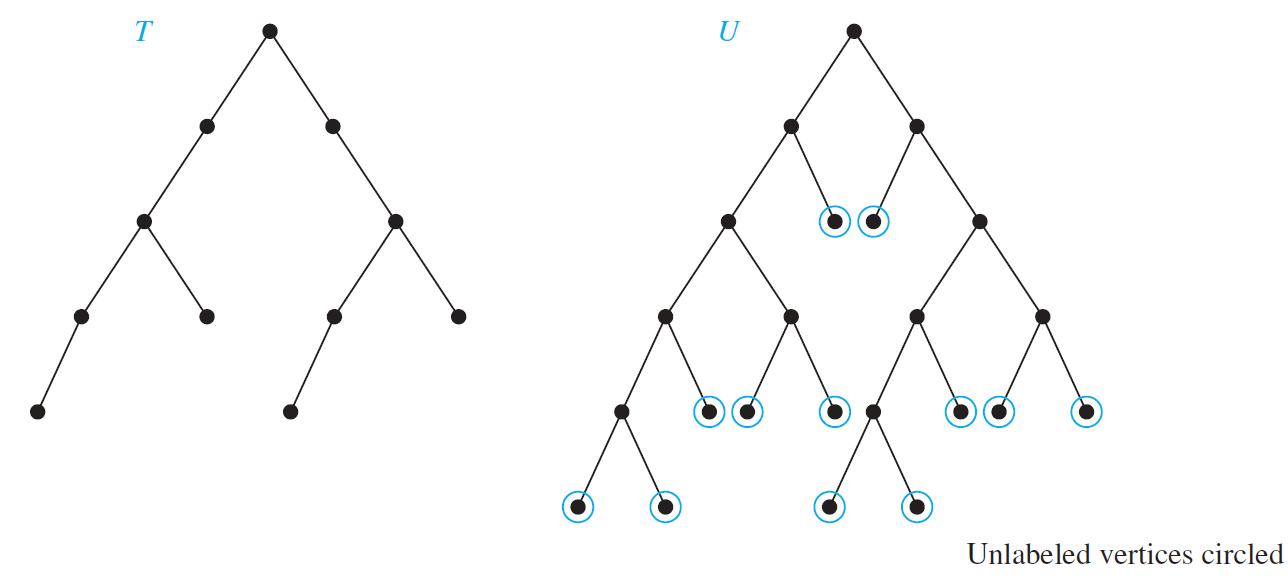
\includegraphics[width=.6\textwidth]{img/ch11.2-figure2.png}
%    \caption{Adding unlabeled vertices to make a binary search tree full.}
%    \label{fig:my_label}
%\end{figure}

%The most comparisons needed to add a new item is the length of the longest path in $U$ from the root to a leaf. The internal vertices of $U$ are the vertices of $T$. It follows that $U$ has $n$ internal vertices. We can now use part $(ii)$ of Theorem 4 in Section 1 to conclude that $U$ has $n + 1$ leaves. 

%Using Corollary 1 of Section 1, we see that the height of $U$ is greater than or equal to $h = \lceil \log_2 (n + 1) \rceil$. So, there must exist an item that requires at least $\lceil \log_2 (n + 1) \rceil$ comparisons to be added to the tree. Note that if $U$ is balanced, its height is $\lceil \log_2 (n + 1) \rceil$ (by Corollary 1 of Section 11). Thus, if a binary search tree is balanced, locating or adding an item requires no more than $\lceil \log_2 (n + 1) \rceil$ comparisons. A binary search tree can become unbalanced as items are added to it. Because balanced binary search trees give optimal worst-case complexity for binary searching, algorithms have been devised that rebalance binary search trees as items are added. 

\section{Tree Traversal}
\setcounter{figure}{0}

\subsection{Introduction}

Ordered rooted trees are often used to store information. We need procedures for visiting each vertex of an ordered rooted tree to access data. Ordered rooted trees can also be used to represent various types of expressions, such as arithmetic expressions involving numbers, variables, and operations.

\subsection{Universal Address Systems}

Procedures for traversing all vertices of an ordered rooted tree rely on the orderings of children. In ordered rooted trees, the children of an internal vertex are shown from left to right in the drawings representing these directed graphs. We will describe one way we can totally order the vertices of an ordered rooted tree. To produce this ordering, we must first label all the vertices. We do this recursively:
\begin{enumerate}
    \item Label the root with the integer 0. Then label its $k$ children (at level 1) from left to right with $1,\ 2,\ 3,\ ...,\ k$.
    \item For each vertex $v$ at level $n$ with label $A$, label its $k_v$ children, as they are drawn from left to right, with $A.1,\ A.2,\ ...,\ A.k_v$.
\end{enumerate}
Following this procedure, a vertex $v$ at level $n$, for $n \geq 1$, is labeled $x_1.x_2. ... .x_n$, where the unique path from the root to $v$ goes through the $x_1st$ vertex at level 1, the $x_2nd$ vertex at level 2, and so on. This labeling is called the \textbf{universal address system} of the ordered rooted tree.

We can totally order the vertices using the lexicographic ordering of their labels in the universal address system. The vertex labeled $x_1.x_2. ... .x_n$ is less than the vertex labeled $y_1.y_2. ... .y_m$ if there is an $i$, $0 \leq i \leq n$, with $x_1 = y_1, x_2 = y_2, ..., x_{i-1} = y_{i-1}$, and $x_i < y_i$; or if $n < m$ and $x_i = y_i$ for $i = 1, 2, ..., n$.

\begin{figure}[h!]
    \centering
    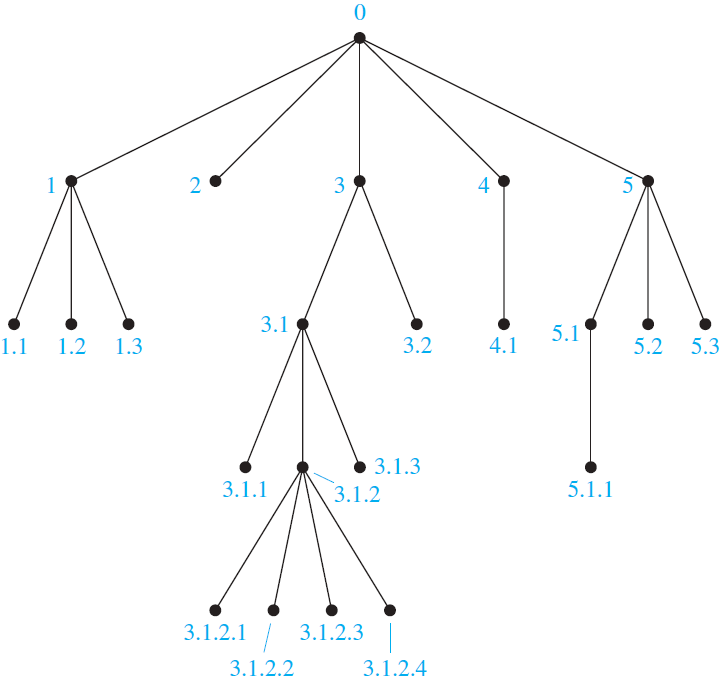
\includegraphics[width=.6\textwidth]{img/ch11.3-figure1.png}
    \caption{The universal address system of an ordered rooted tree}
    \label{fig:ch11.3}
\end{figure}

\subsection{Traversal Algorithms}

Procedures for systematically visiting every vertex of an ordered rooted tree are called \textbf{traversal algorithms}. We will describe three of the most commonly used such algorithms, \textbf{preorder traversal}, \textbf{inorder traversal}, and \textbf{postorder traversal}. Each of these algorithms can be defined recursively.

\newpage
\subsubsection{Preorder}

We first define preorder traversal.

\begin{mybox}{blue}{\textbf{Definition 1}}
Let $T$ be an ordered rooted tree with root $r$. If $T$ consists only of $r$, then $r$ is the \textit{preorder traversal} of $T$. Otherwise, suppose that $T_1,\ T_2,\ ...,\ T_n$ are the subtrees at $r$ from left to right in $T$. The \textit{preorder traversal} begins by visiting $r$. It continues by traversing $T_1$ in preorder, then $T_2$ in preorder, and so on, until $T_n$ is traversed in preorder.
\end{mybox}

\begin{figure}[h!]
    \centering
    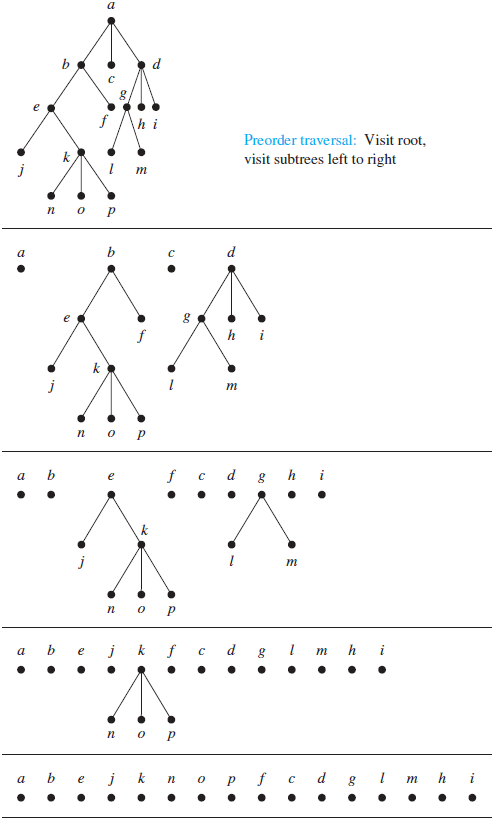
\includegraphics[width=.7\textwidth]{img/ch11.3-figure4.png}
    \caption{The preorder traversal of $T$.}
    \label{fig:my_label}
\end{figure}

\subsubsection{Inorder}

We will now define inorder traversal.

\begin{mybox}{blue}{\textbf{Definition 2}}
Let $T$ be an ordered rooted tree with root $r$. If $T$ consists only of $r$, then $r$ is the \textit{inorder traversal} of $T$. Otherwise, suppose that $T_1,\ T_2,\ ...,\ T_n$ are the subtrees at $r$ from left to right. The \textit{inorder traversal} begins by traversing $T_1$ in inorder, then visiting $r$. It continues by traversing $T_2$ in inorder, then $T_3$ in inorder, ..., and finally $T_n$ in inorder.
\end{mybox}

\begin{figure}[h!]
    \centering
    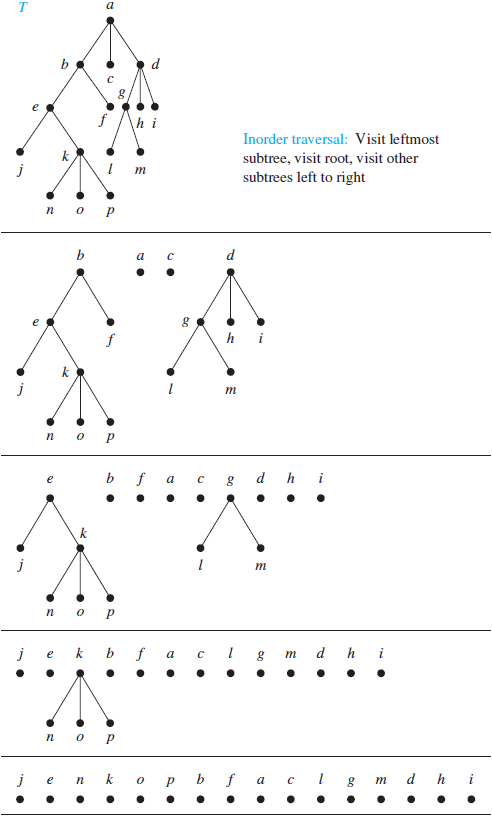
\includegraphics[width=.7\textwidth]{img/ch11.3-figure6.png}
    \caption{The inorder traversal of $T$.}
    \label{fig:my_label}
\end{figure}

\subsubsection{Postorder}

We now define postorder traversal.

\begin{mybox}{blue}{\textbf{Definition 3}}
Let $T$ be an ordered rooted tree with root $r$. If $T$ consists only of $r$, then $r$ is the \textit{postorder traversal} of $T$. Otherwise, suppose that $T_1,\ T_2,\ ...,\ T_n$ are the subtrees at $r$ from left to right. The \textit{postorder traversal} begins by traversing $T_1$ in postorder, then $T_2$ in postorder, ..., then $T_n$ in postorder, and ends by visiting $r$.
\end{mybox}

\begin{figure}[h!]
    \centering
    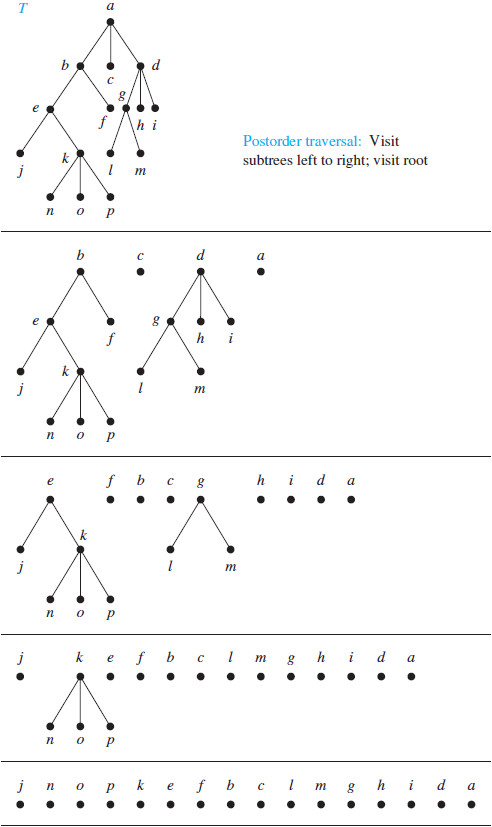
\includegraphics[width=.65\textwidth]{img/ch11.3-figure8.png}
    \caption{The inorder traversal of $T$.}
    \label{fig:my_label}
\end{figure}


Algorithms for traversing ordered rooted trees in preorder, inorder, or postorder are most easily expressed recursively.

\begin{algorithm}
\caption{Preorder Traversal}
\begin{algorithmic}[1]
\Procedure {$preorder$($T$: ordered rooted tree)}{}
\State $r$ := root of $T$
\State list $r$
\For {each child $c$ of $r$ from left to right}
\State $T(c)$ := subtree with $c$ as its root
\State $preorder(T(c))$
\EndFor
\EndProcedure
\end{algorithmic}
\end{algorithm}

\begin{algorithm}
\caption{Inorder Traversal}
\begin{algorithmic}[1]
\Procedure {$inorder$($T$: ordered rooted tree)}{}
\State $r$ := root of $T$
\If {$r$ is a leaf} {list $r$}
\Else
\State $l$ := first child of $r$ from left to right
\State $T(l)$ := subtree with $l$ as its root
\State $inorder(T(l))$
\State list $r$
\For{each child $c$ of $r$ except for $l$ from left to right}
\State $T(c)$ := subtree with $c$ as its root
\State $inorder(T(c))$
\EndFor
\EndIf
\EndProcedure
\end{algorithmic}
\end{algorithm}

\begin{algorithm}[h!]
\caption{Postorder Traversal}
\begin{algorithmic}[1]
\Procedure {$postorder$($T$: ordered rooted tree)}{}
\State $r$ := root of $T$
\For {each child $c$ of $r$ from left to right}
\State $T(c)$ := subtree with $c$ as its root
\State $preorder(T(c))$
\EndFor
\State list $r$
\EndProcedure
\end{algorithmic}
\end{algorithm}


Both the \textit{preorder traversal} and the \textit{postorder traversal} \textit{encode the structure of an ordered rooted tree} when the number of children of each vertex is specified. That is, an ordered rooted tree is uniquely determined when we specify a list of vertices generated by a preorder traversal or by a postorder traversal of the tree, together with the number of children of each vertex. 

In particular, \textit{both a preorder traversal and a postorder traversal encode the structure of a full ordered $m$-ary tree}. However, when the number of children of vertices is not specified, neither a preorder traversal nor a postorder traversal encodes the structure of an ordered rooted tree.

\subsubsection{Uses of Inorder, Preorder, and Postorder Traversals}

Tree traversals have many applications and they play a key role in the implementation of many algorithms. 

Binary ordered trees can be used to represent well-formed expressions of objects and operations. Preorder, postorder, and inorder traversals of these trees yield the prefix, postfix, and infix notations of expressions, which can then be used in applications.

Before we turn our attention to that use of tree traversals,
we will provide useful guidance about the practical use of tree traversals.\\

When efficiency is not an issue, the vertices of a tree can be visited in any order, so long as each node is visited exactly once. However, for other applications we may need to visit vertices in an order that preserves a specific relationship. Also, when efficiency is important, the most efficient traversal method for that application should be used. A general principle for deciding the traversal to use is to explore the vertices of interest as soon as possible.

\textit{Preorder traversal is the best choice for applications where internal vertices must be explored before leaves}. Preorder traversals are also used to make copies of binary search trees.

\textit{Postorder traversal is the best choice for applications where leaves need to be explored before internal vertices}. Postorder explores leaves before internal vertices, so it is the best choice for deleting a tree because the vertices below the root of a subtree can be removed before the root of the subtree. 

Topological sorting is an example of an algorithm that can be efficiently implemented using postorder traversal.\\

An inorder traversal of a binary search tree, visits the vertices in ascending order of their key values. Such a traversal creates a sorted list of the data in a binary tree.

\subsection{Infix, Prefix, and Postfix Notation}

We can represent complicated expressions, such as compound propositions, combinations of sets, and arithmetic expressions using ordered rooted trees. For instance, consider the representation of an arithmetic expression involving the operators + (addition), - (subtraction), * (multiplication), / (division), and ↑ (exponentiation).We will use parentheses to indicate the order of the operations. \textit{An ordered rooted tree can be used to represent such expressions, where the internal vertices represent operations, and the leaves represent the variables or numbers.} Each operation operates on its left and right subtrees (in that order).

\begin{example}
What is the ordered rooted tree that represents the expression $((x + y)↑2) + ((x - 4)/3)$?

\textbf{Solution:}

The binary tree for this expression can be built from the bottom up. First, a subtree for the expression $x + y$ is constructed. Then this is incorporated as part of the larger subtree representing $(x + y)↑2$. Also, a subtree for $x - 4$ is constructed, and then this is incorporated into a subtree representing $(x - 4)/3$. Finally the subtrees representing $(x + y) ↑ 2$ and $(x - 4)/3$ are combined to form the ordered rooted tree representing $((x + y) ↑ 2) + ((x - 4)/3)$. These steps are shown in Figure 5.
\end{example}

\begin{figure}[h!]
    \centering
    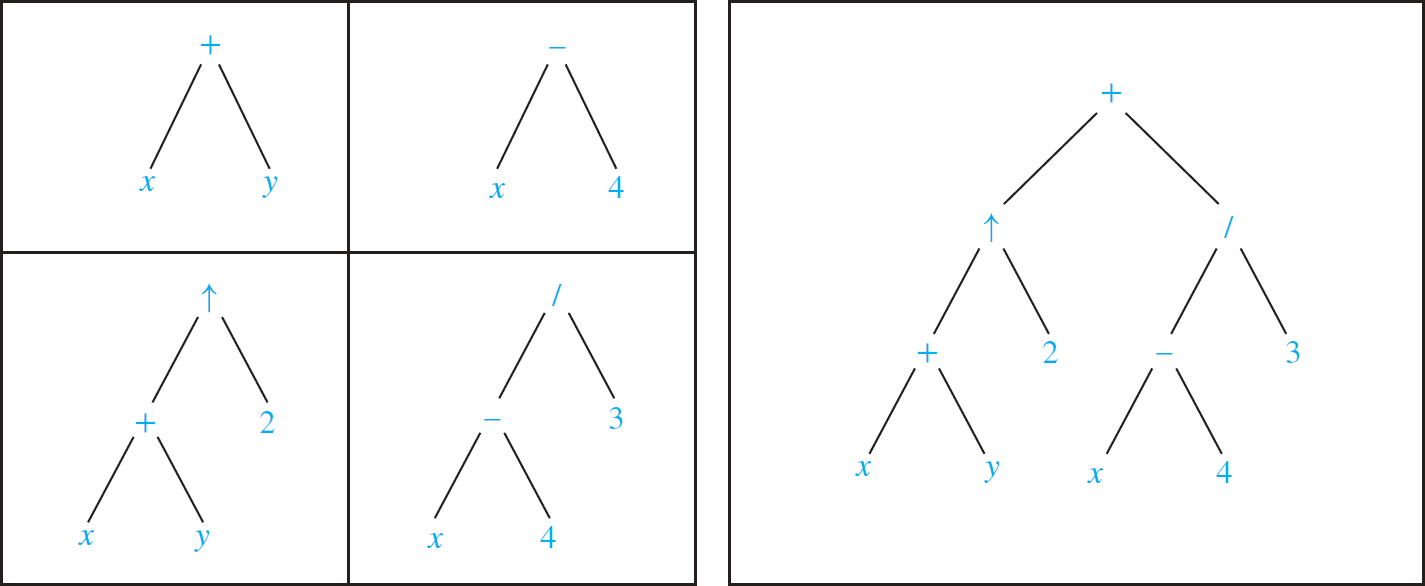
\includegraphics[width=.7\textwidth]{img/ch11.3-figure10.png}
    \caption{A binary tree representing $((x + y) ↑ 2) + ((x - 4)/3)$.}
    \label{fig:ch_11.3}
\end{figure}

An inorder traversal of the binary tree representing an expression produces the original expression with the elements and operations in the same order as they originally occurred, except for unary operations, which instead immediately follow their operands. To make expressions unambiguous it is necessary to include parentheses in the inorder traversal whenever we encounter an operation. The fully parenthesized expression obtained in this way is said to be in \textbf{infix form}.

We obtain the \textbf{prefix form} of an expression when we traverse its rooted tree in \textit{preorder}. Expressions written in prefix form are said to be in \textbf{Polish notation}. An expression in prefix notation (where each operation has a specified number of operands), is unambiguous, so no parentheses are needed in such an expression.

\begin{example}
What is the prefix form for $((x + y) ↑ 2) + ((x - 4)/3)$?

\textbf{Solution:}
We obtain the prefix form for this expression by traversing the binary tree that represents it in preorder, shown in Figure 5. This produces $+\ ↑\ +\ x\ y\ 2\ /\ -\ x\ 4\ 3$.
\end{example}


\begin{figure}[h!]
\begin{minipage}[c]{0.45\textwidth}
    \centering
    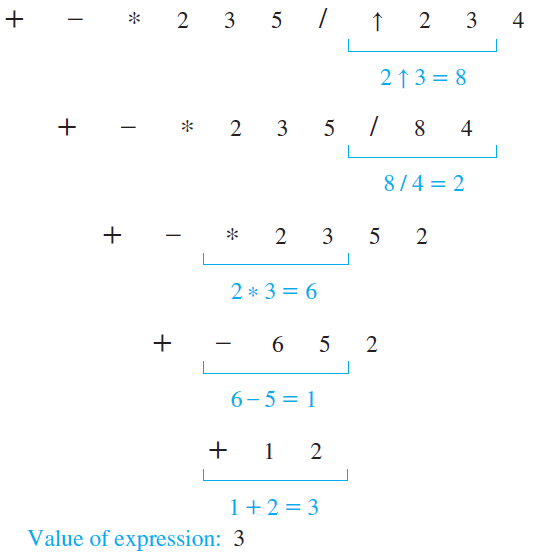
\includegraphics[width=\textwidth]{img/ch11.3-figure12.png}
    \caption{Evaluating a prefix expression.}
\end{minipage}\hfill
\begin{minipage}[c]{0.45\textwidth}
    \centering
    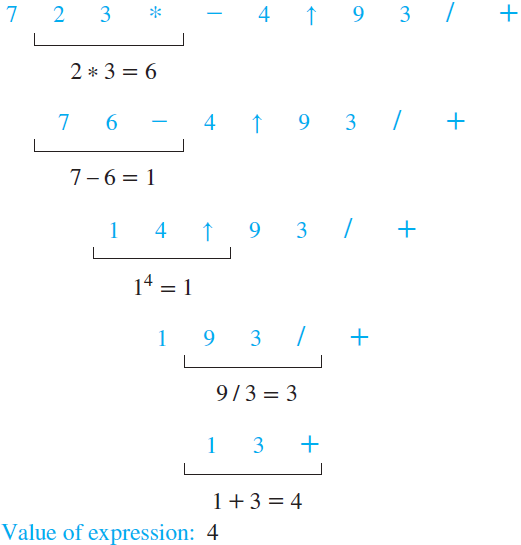
\includegraphics[width=\textwidth]{img/ch11.3-figure13.png}
    \caption{Evaluating a postfix expression.}
\end{minipage}\hfill
\end{figure}

\newpage
In the prefix form of an expression, a binary operator, such as +, precedes its two operands. Hence, we can evaluate an expression in prefix form by working from right to left. When we encounter an operator, we perform the corresponding operation with the two operands immediately to the right of this operand. Also, whenever an operation is performed, we consider the result a new operand.

\begin{example}
What is the value of the prefix expression $+\ -\ *\ 2\ 3\ 5\ /\ ↑\ 2\ 3\ 4$?

\textbf{Solution:}
The steps used to evaluate this expression by working right to left, and performing operations using the operands on the right, are shown in Figure 6. The value of this expression is 3.
\end{example}


We obtain the \textbf{postfix form} of an expression by traversing its binary tree in postorder. Expressions written in postfix form are said to be in \textbf{reverse Polish notation}. Expressions in reverse Polish notation are unambiguous, so parentheses are not needed. The verification of this is left to the reader.

\begin{example}
What is the postfix form of the expression $((x + y) ↑ 2) + ((x - 4)/3)$?

\textbf{Solution:}
The postfix form of the expression is obtained by carrying out a postorder traversal of the binary tree for this expression, shown in Figure 5. This produces the postfix expression: $x\ y\ +\ 2\ ↑\ x\ 4\ -\ 3\ /\ +$.
\end{example}

In the postfix form of an expression, a binary operator follows its two operands. So, to evaluate an expression from its postfix form, work from left to right, carrying out operations whenever an operator follows two operands. After an operation is carried out, the result of this operation becomes a new operand.

\begin{example}
What is the value of the postfix expression $7\ 2\ 3\ *\ -\ 4\ ↑\ 9\ 3\ /\ +$?

\textbf{Solution:}
The steps used to evaluate this expression by starting at the left and carrying out operations when two operands are followed by an operator are shown in Figure 7. The value of this expression is 4.
\end{example}

Rooted trees can be used to represent other types of expressions, such as those representing compound propositions and combinations of sets. In these examples unary operators, such as the negation of a proposition, occur. To represent such operators and their operands, a vertex representing the operator and a child of this vertex representing the operand are used.


\begin{figure}[h!]
    \centering
    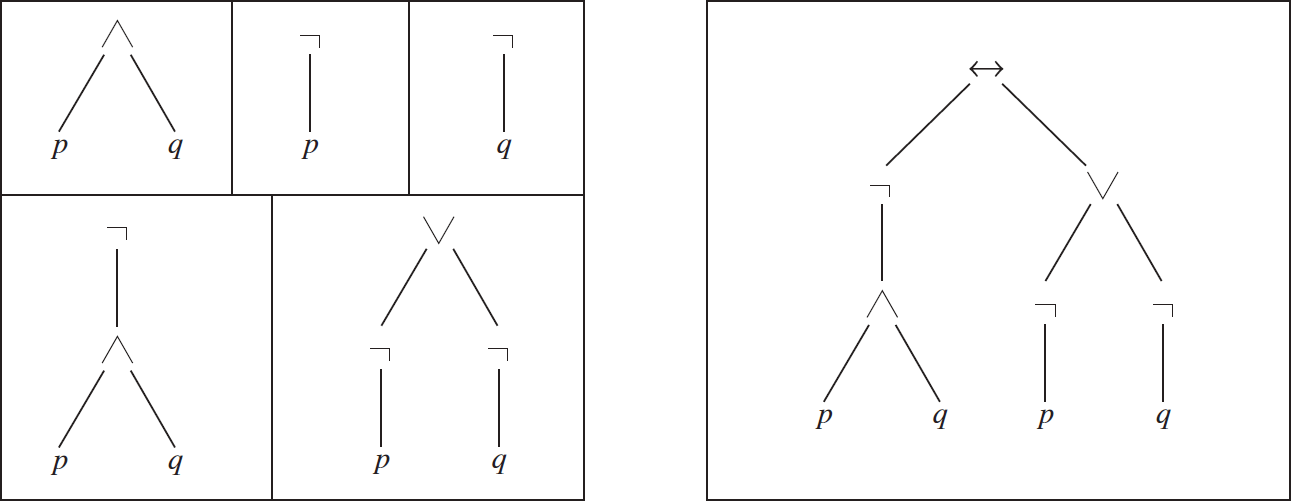
\includegraphics[width=.8\textwidth]{img/ch11.3-figure14.png}
    \caption{Constructing the rooted tree for a compound proposition.}
    \label{fig:ch_11.3}
\end{figure}


\begin{example}
Find the ordered rooted tree representing the compound proposition $(\neg(p \land q)) \leftrightarrow (\neg p \lor \neg q)$. Then use this rooted tree to find the prefix, postfix, and infix forms of this expression.

\textbf{Solution:}
The rooted tree for this compound proposition is constructed from the bottom up. First, subtrees for $\neg p$ and $\neg q$ are formed (where $\neg$ is considered a unary operator). Also, a subtree for $p \land q$ is formed. Then subtrees for $\neg (p \land q)$ and $(\neg p) \lor (\neg q)$ are constructed. Finally, these two subtrees are used to form the final rooted tree. The steps of this procedure are shown in Figure 8.\\

The prefix, postfix, and infix forms of this expression are found by traversing this rooted tree in preorder, postorder, and inorder (including parentheses), respectively. These traversals give $\leftrightarrow \neg \land p\ q \lor \neg\  p\ \neg\ q$, $p\ q \land \neg\ p\ \neg\ q\ \neg\ \lor \leftrightarrow$, and $(\neg  (p \land q)) \leftrightarrow ((\neg p) \lor (\neg q))$, respectively.
\end{example}

Because prefix and postfix expressions are unambiguous and because they can be evaluated easily without scanning back and forth, they are used extensively in computer science. Such expressions are especially useful in the construction of compilers.


\section{Spanning Trees}
\setcounter{figure}{0}
\setcounter{algorithm}{0}

\subsection{Introduction}

Consider the system of roads in Maine represented by the simple graph shown in Figure 1(a). The only way the roads can be kept open in the winter is by frequently plowing them. The highway department wants to plow the fewest roads so that there will always be cleared roads connecting any two towns. How can this be done?

At least five roads must be plowed to ensure that there is a path between any two towns. Figure 1(b) shows one such set of roads. Note that the subgraph representing these roads is a tree, because it is connected and contains six vertices and five edges. 

This problem was solved with a connected subgraph with the minimum number of edges containing all vertices of the original simple graph. Such a graph must be a tree.

\begin{figure}[h!]
    \centering
    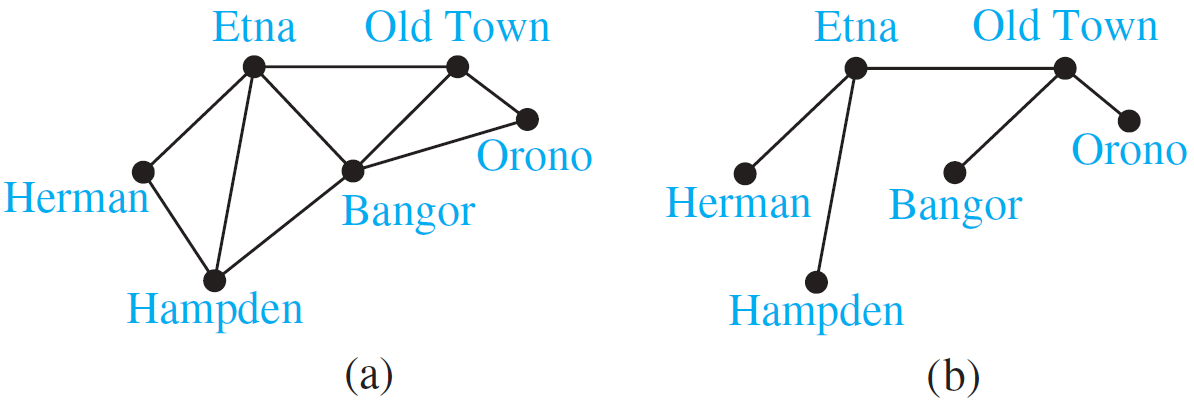
\includegraphics[width=.7\textwidth]{img/ch11.4-figure1.png}
    \caption{(a) A road system and (b) a set of
roads to plow.}
    \label{fig:my_label}
\end{figure}

\begin{definition}
{1}
Let $G$ be a simple graph. A spanning tree of $G$ is a subgraph of $G$ that is a tree containing every vertex of $G$.
\end{definition}

\textit{A simple graph with a spanning tree must be connected, because there is a path in the spanning tree between any two vertices}. The converse is also true; that is, \textit{every connected simple graph has a spanning tree}.

\begin{theorem}
{1}
A simple graph is connected if and only if it has a spanning tree.
\end{theorem}

\begin{proof}
First, suppose that a simple graph $G$ has a spanning tree $T$. $T$ contains every vertex of $G$. Furthermore, there is a path in $T$ between any two of its vertices. Because $T$ is a subgraph of $G$, there is a path in $G$ between any two of its vertices. Hence, $G$ is connected.

Now suppose that $G$ is connected. If $G$ is not a tree, it must contain a simple circuit. Remove an edge from one of these simple circuits. The resulting subgraph has one fewer edge but still contains all the vertices of $G$ and is connected. This subgraph is still connected because when two vertices are connected by a path containing the removed edge, they are connected by a path not containing this edge. We can construct such a path by inserting into the original path, at the point where the removed edge once was, the simple circuit with this edge removed. If this subgraph is not a tree, it has a simple circuit; so as before, remove an edge that is in a simple circuit. Repeat this process until no simple circuits remain. This is possible because there are only a finite number of edges in the graph. The process terminates when no simple circuits remain. A tree is produced because the graph stays connected as edges are removed. This tree is a spanning tree because it contains every vertex of $G$.
\end{proof}

\subsection{Depth-First Search}

The proof of Theorem 1 gives an algorithm for finding spanning trees by removing edges from simple circuits. This algorithm is inefficient, because it requires that simple circuits be identified. Instead of constructing spanning trees by removing edges, spanning trees can be built up by successively adding edges. Two algorithms based on this principle will be presented here.

We can build a spanning tree for a connected simple graph using \textbf{depth-first search}. We will form a rooted tree, and the spanning tree will be the underlying undirected graph of this rooted tree. Arbitrarily choose a vertex of the graph as the root. Form a path starting at this vertex by successively adding vertices and edges, where each new edge is incident with the last vertex in the path and a vertex not already in the path. Continue adding vertices and edges to this path as long as possible. If the path goes through all vertices of the graph, the tree consisting of this path is a \textit{spanning tree}. 

However, if the path does not go through all vertices, more vertices and edges must be added. Move back to the next to last vertex in the path, and, if possible, form a new path starting at this vertex passing through vertices that were not already visited. If this cannot be done, move back another vertex in the path, that is, two vertices back in the path, and try again.

Repeat this procedure, beginning at the last vertex visited, moving back up the path one vertex at a time, forming new paths that are as long as possible until no more edges can be added. Because the graph has a finite number of edges and is connected, this process ends with the production of a spanning tree. Each vertex that ends a path at a stage of the algorithm will be a leaf in the rooted tree, and each vertex where a path is constructed starting at this vertex will be an internal vertex.

The recursive nature of this procedure should be noted. Also, note that if the vertices in the graph are ordered, the choices of edges at each stage of the procedure are all determined when we always choose the first vertex in the ordering that is available. However, we will not always explicitly order the vertices of a graph.

Depth-first search is also called \textbf{backtracking}, because the algorithm returns to vertices previously visited to add paths.


\begin{example}
Use depth-first search to find a spanning tree for the graph $G$ shown in Figure 2.

\textbf{Solution:} The steps used by depth-first search to produce a spanning tree of $G$ are shown in Examples Figure 3. We arbitrarily start with the vertex $f$ . 

A path is built by successively adding edges incident with vertices not already in the path, as long as this is possible. This produces a path $f,\ g,\ h,\ k,\ j$ (note that other paths could have been built). 

Next, backtrack to $k$. There is no path beginning at $k$ containing vertices not already visited. So we backtrack to $h$. Form the path $h,\ i$. Then backtrack to $h$, and then to $f$. From $f$ build the path $f,\ d,\ e,\ c,\ a$. Then backtrack to $c$ and form the path $c$, $b$. This produces the spanning tree.
\end{example}

\begin{figure}[h!]
\begin{minipage}[c]{0.40\textwidth}
    \centering
    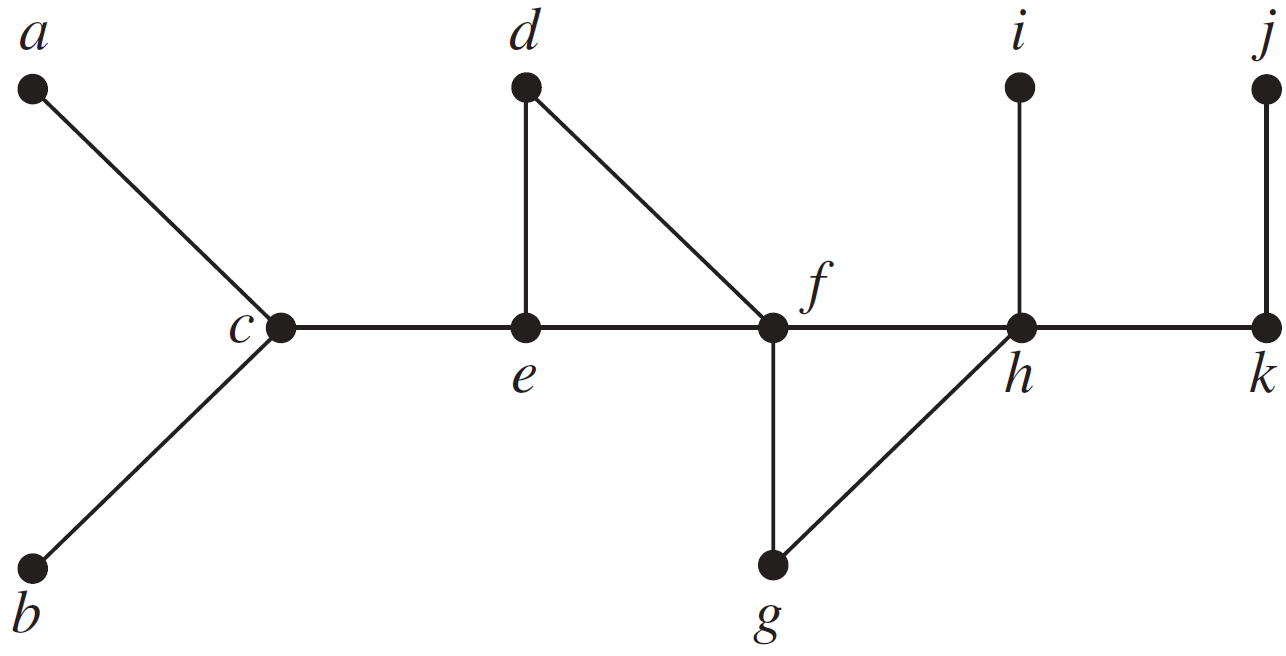
\includegraphics[width=\textwidth]{img/ch11.4-figure6.png}
    \caption{The graph $G$.}
\end{minipage}\hfill
\begin{minipage}[c]{0.55\textwidth}
    \centering
    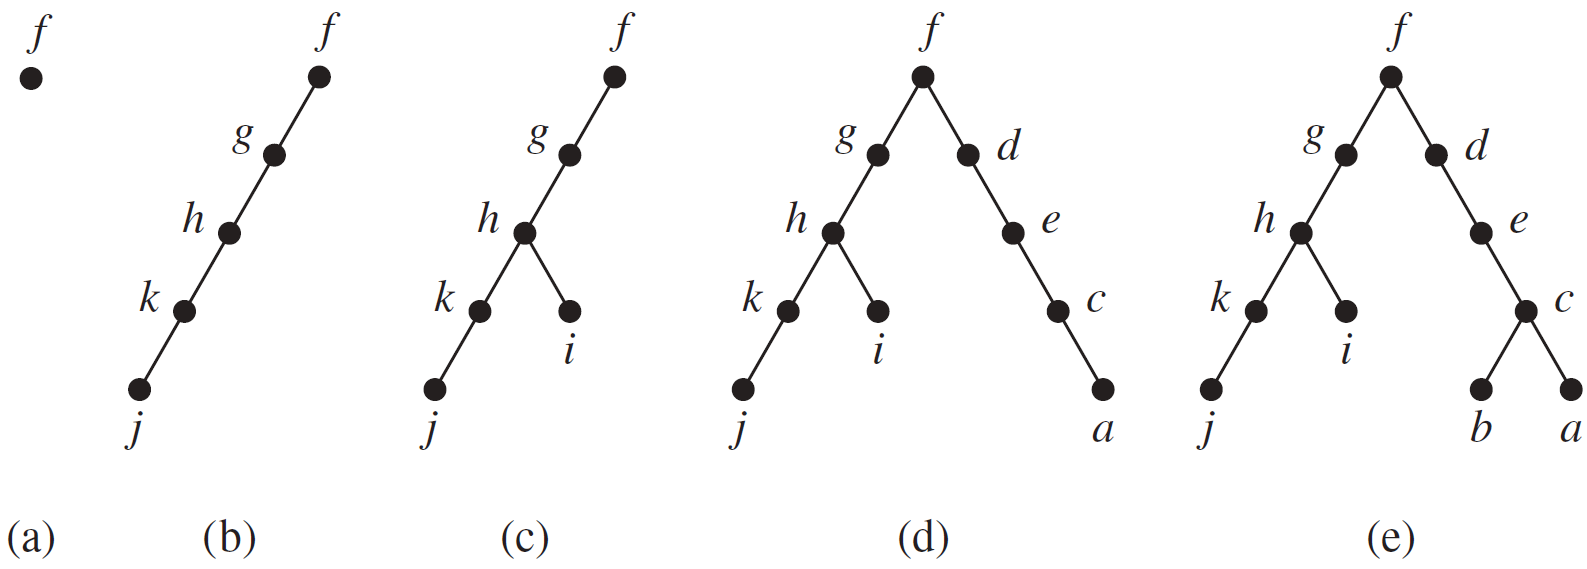
\includegraphics[width=\textwidth]{img/ch11.4-figure7.png}
    \caption{Depth-first search of $G$.}
\end{minipage}\hfill
\end{figure}

The edges selected by depth-first search of a graph are called \textbf{tree edges}. All other edges of the graph must connect a vertex to an ancestor or descendant of this vertex in the tree. These edges are called \textbf{back edges}.

In Algorithm 1 we construct the spanning tree of a graph $G$ with vertices $v_1,\ ...,\ v_n$ by first selecting the vertex $v_1$ to be the root. We initially set $T$ to be the tree with just this one vertex. At each step we add a new vertex to the tree $T$ together with an edge from a vertex already in $T$ to this new vertex and we explore from this new vertex. Note that at the completion of the algorithm, $T$ contains no simple circuits because no edge is ever added that connects two vertices in the tree. Moreover, $T$ remains connected as it is built. (These last two observations can be easily proved via mathematical induction.) Because $G$ is connected, every vertex in $G$ is visited by the algorithm and is added to the tree. It follows that $T$ is a spanning tree of $G$.

\begin{algorithm}
\caption{Depth-First Search}
\begin{algorithmic}
\Procedure{$DFS$}{$G$: connected graph with vertices $v_1,\ v_2,\ ...\ v_n$}
\State $T$ := tree consisting only of the vertex $v_1$
\State $visit(v_1)$
\EndProcedure
\\
\Procedure{$visit$}{$v$: vertex of $G$}
\For{each vertex $w$ adjacent to $v$ and not yet in $T$}
\State add vertex $w$ and edge $\{v,w\}$ to $T$
\State $visit(w)$
\EndFor
\EndProcedure
\end{algorithmic}
\end{algorithm}

We now analyze the computational complexity of the depth-first search algorithm. The key observation is that for each vertex $v$, the procedure $visit(v)$ is called when the vertex $v$ is first encountered in the search and it is not called again. Assuming that the adjacency lists for $G$ are available, no computations are required to find the vertices adjacent to $v$. As we follow the steps of the algorithm, we examine each edge at most twice to determine whether to add this edge and one of its endpoints to the tree. Consequently, the procedure $DFS$ constructs a spanning tree using $O(e)$, or $O(n^2)$, steps where $e$ and $n$ are the number of edges and vertices in $G$, respectively. [Note that a step involves examining a vertex to see whether it is already in the spanning tree as it is being built and adding this vertex and the corresponding edge if the vertex is not already in the tree. We have also made use of the inequality $e \leq n(n - 1)/2$, which holds for any simple graph.] 

Depth-first search can be used as the basis for algorithms that solve many different problems. For example, it can be used to find paths and circuits in a graph, it can be used to determine the connected components of a graph, and it can be used to find the cut vertices of a connected graph. 

\subsection{Breadth-First Search}

We can also produce a spanning tree of a simple graph by the use of breadth-first search. Again, a rooted tree will be constructed, and the underlying undirected graph of this rooted tree forms the spanning tree. 

Arbitrarily choose a root from the vertices of the graph. Then add all edges incident to this vertex. The new vertices added at this stage become the vertices at level 1 in the spanning tree. Arbitrarily order them. 

Next, for each vertex at level 1, visited in order, add each edge incident to this vertex to the tree as long as it does not produce a simple circuit. Arbitrarily order the children of each vertex at level 1. This produces the vertices at level 2 in the tree. Follow the same procedure until all the vertices in the tree have been added. 

The procedure ends because there are only a finite number of edges in the graph. A spanning tree is produced because we have produced a tree containing every vertex of the graph.

\begin{example}
Use breadth-first search to find a spanning tree for the graph shown in Figure 4.

\textbf{Solution:}
The steps of the breadth-first search procedure are shown in Figure 5. We choose the vertex $e$ to be the root. Then we add edges incident with all vertices adjacent to $e$, so edges from $e$ to $b,\ d,\ f$, and $i$ are added. These four vertices are at level 1 in the tree. 

Next, add the edges from these vertices at level 1 to adjacent vertices not already in the tree. Hence, the edges from $b$ to $a$ and $c$ are added, as are edges from $d$ to $h$, from $f$ to $j$ and $g$, and from $i$ to $k$. The new
vertices $a,\ c,\ h,\ j,\ g$, and $k$ are at level 2.

Next, add edges from these vertices to adjacent vertices not already in the graph. This adds edges from $g$ to $l$ and from $k$ to $m$.
\end{example}

\begin{figure}[h!]
\begin{minipage}[c]{0.2\textwidth}
    \centering
    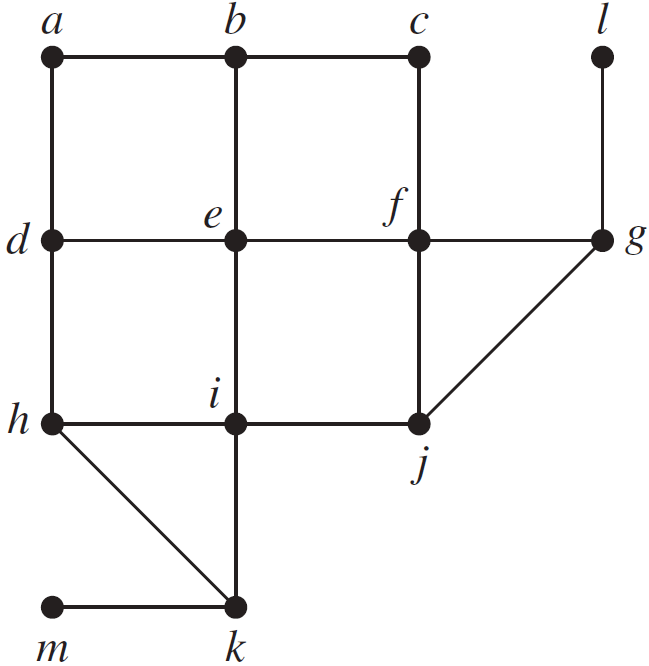
\includegraphics[width=\textwidth]{img/ch11.4-figure9.png}
    \caption{A graph $G$.}
\end{minipage}\hfill
\begin{minipage}[c]{0.75\textwidth}
    \centering
    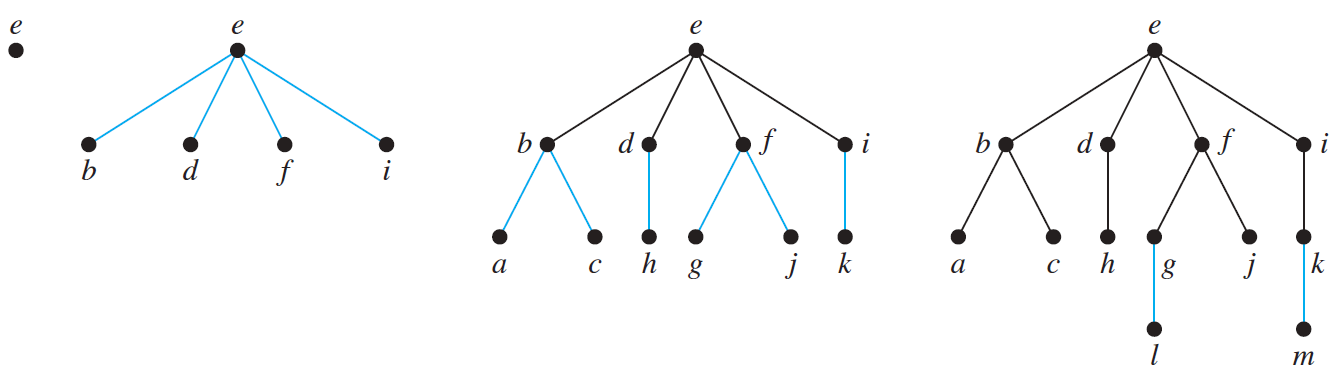
\includegraphics[width=\textwidth]{img/ch11.4-figure10.png}
    \caption{Breadth-first search of $G$.}
\end{minipage}\hfill
\end{figure}

We describe breadth-first search in pseudocode as Algorithm 2. In this algorithm, we assume the vertices of the connected graph $G$ are ordered as $v_1,\ v_2,\ ...,\ v_n$. In the algorithm we use the term "process" to describe the procedure of adding new vertices, and corresponding edges, to the tree adjacent to the current vertex being processed as long as a simple circuit is not produced.

\begin{algorithm}
\caption{Breadth-First Search}
\begin{algorithmic}
\Procedure{$BFS$}{$G$: connected graph with vertices $v_1,\ v_2,\ ...,\ v_n$}
\State $T$ := tree consisting only of vertex $v_1$
\State $L$ := empty list
\State put $v_1$ in the list $L$ of unprocessed vertices
\While{$L$ is not empty}
\State remove the first vertex, $v$, from $L$
\For{each neighbor $w$ of $v$}
\If{$w$ is not in $L$ and not in $T$}
\State add $w$ to the end of the list $L$
\State add $w$ and edge $\{v, w\}$ to $T$
\EndIf
\EndFor
\EndWhile
\EndProcedure
\end{algorithmic}
\end{algorithm}

\newpage
We now analyze the computational complexity of breadth-first search. For each vertex $v$ in the graph we examine all vertices adjacent to $v$ and we add each vertex not yet visited to the tree $T$. Assuming we have the adjacency lists for the graph available, no computation is required to determine which vertices are adjacent to a given vertex. As in the analysis of the depth-first search algorithm, we see that we examine each edge at most twice to determine whether we should add this edge and its endpoint not already in the tree. It follows that the breadth-first search algorithm uses $O(e)$ or $O(n^2)$ steps.

Breadth-first search is one of the most useful algorithms in graph theory. In particular, it can serve as the basis for algorithms that solve a wide variety of problems. For example, algorithms that find the connected components of a graph, that determine whether a graph is bipartite, and that find the path with the fewest edges between two vertices in a graph can all be built using breadth-first search.

\subsubsection{Breadth-First Search versus Depth-First Search}

We have introduced two widely used algorithms for constructing spanning trees of graphs, \textit{breadth-first search (BFS)} and \textit{depth-first search (DFS)}. Both algorithms can be used to produce a spanning tree when given a connected graph. But why might it be better to use one rather than the other?\\

Although both BFS and DFS can be used to solve the same problems, there are theoretical and practical reasons for choosing between them. To solve a particular type of problem, one of these search algorithms can be easier to apply, or can provide more insight, than the other. 

For some problems, BFS can be easier to use than DFS because BFS partitions the vertices of a graph into levels, which tell us how far away vertices are from the root. Also, edges connect vertices at the same level or at adjoining levels.

On the other hand, there are many types of problems that are more naturally solved using DFS. Generally, DFS is a better choice when we need to explore a graph by exploring deeper rather than by exploring the graph systematically level by level. The structure obtained when using DFS can also be used when solving problems.\\

Both BFS and DFS are extensively used in practice. The choice for which to use often depends on implementation details, such as the data structures used. Time and space considerations are paramount, especially when the problems being solved involved huge graphs. Also, keep in mind that we often solve problems using graph searching without completing the task of finding a spanning tree. 

When we use BFS on a graph that is dense, we spend a lot of time and use a lot of space to explore the graph level by level. In such situations, it can be preferable to use DFS to quickly reach vertices far away from the root. For a sparse graph, however, it may be more efficient to explore a graph level by level.

\subsection{Backtracking Applications}

There are problems that can be solved only by performing an exhaustive search of all possible solutions. One way to search systematically for a solution is to use a decision tree, where each internal vertex represents a decision and each leaf a possible solution. To find a solution via backtracking, first make a sequence of decisions in an attempt to reach a solution as long as this is possible. The sequence of decisions can be represented by a path in the decision tree. Once it is known that no solution can result from any further sequence of decisions, backtrack to the parent of the current vertex and work toward a solution with another series of decisions, if this is possible. The procedure continues until a solution is found, or it is established that no solution exists.

\textit{(Check the examples starting from page 828 to 830 in the book)}.

\subsection{Depth-First Search in Directed Graphs}

We can easily modify both \textit{depth-first search} and \textit{breadth-first search} so that they can run given a directed graph as input. However, the output will not necessarily be a spanning tree, but rather a spanning forest. In both algorithms we can add an edge only when it is directed away from the vertex that is being visited and to a vertex not yet added. If at a stage of either algorithm we find that no edge exists starting at a vertex already added to one not yet added, the next vertex added by the algorithm becomes the root of a new tree in the spanning forest.

\begin{example}
What is the output of depth-first search given the graph $G$ shown in Figure 6(a) as input?

\textbf{Solution:}
We begin the depth-first search at vertex $a$ and add vertices $b,\ c$, and $g$ and the corresponding edges where we are blocked. 

We backtrack to $c$ but we are still blocked, and then backtrack to $b$, where we add vertices $f$ and $e$ and the corresponding edges. Backtracking takes
us all the way back to $a$. 

    We then start a new tree at $d$ and add vertices $h$, $l$, $k$, and $j$ and the corresponding edges. 

We backtrack to $k$, then $l$, then $h$, and back to $d$. 

Finally, we start a new tree at $i$, completing the depth-first search. The output is shown in Figure 6(b).
\end{example}

\begin{figure}[h!]
    \centering
    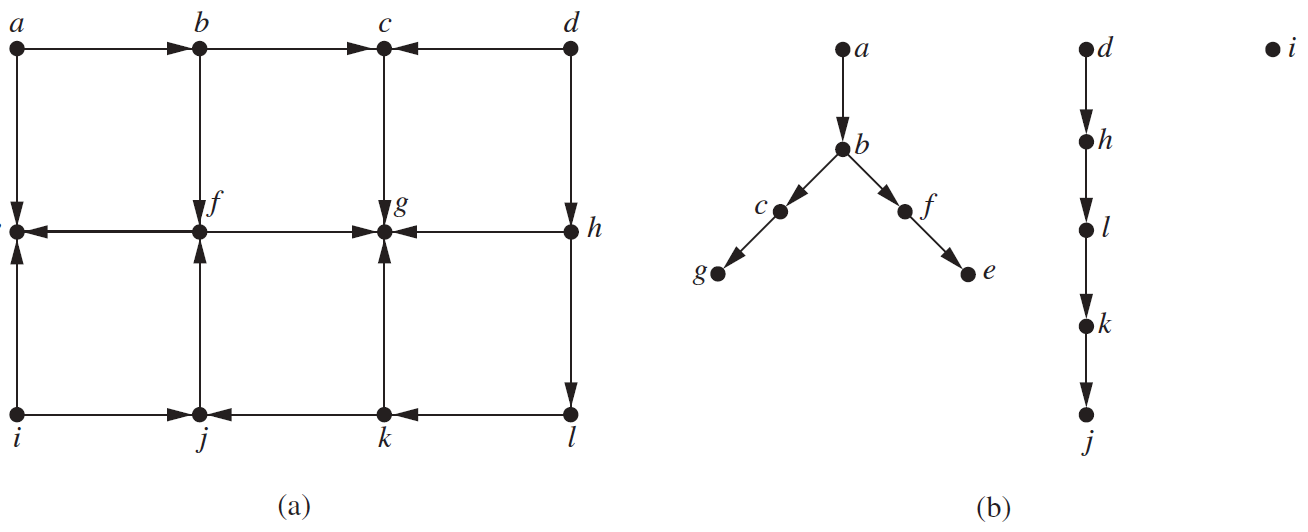
\includegraphics[width=\textwidth]{img/ch11.4-figure14.png}
    \caption{Depth-first search of a directed graph}
    \label{fig:my_label}
\end{figure}

Depth-first search in directed graphs is the basis of many algorithms. It can be used to determine whether a directed graph has a circuit, it can be used to carry out a topological sort of a graph, and it can also be used to find the strongly connected components of a directed graph.

\textit{(The example 10 in page 831 should be read from text book)}.


\section{Minimum Spanning Trees}
\setcounter{figure}{0}
\setcounter{algorithm}{0}

\subsection{Introduction}

A company plans to build a communications network connecting its five computer centers. Any pair of these centers can be linked with a leased telephone line. Which links should be made to ensure that there is a path between any two computer centers so that the total cost of the network is minimized? We can model this problem using the weighted graph shown in Figure 1, where vertices represent computer centers, edges represent possible leased lines, and the weights on edges are the monthly lease rates of the lines represented by the edges. We can solve this problem by finding a spanning tree so that the sum of the weights of the edges of the tree is minimized. Such a spanning tree is called a \textbf{minimum spanning tree}.

\begin{figure}[h!]
    \centering
    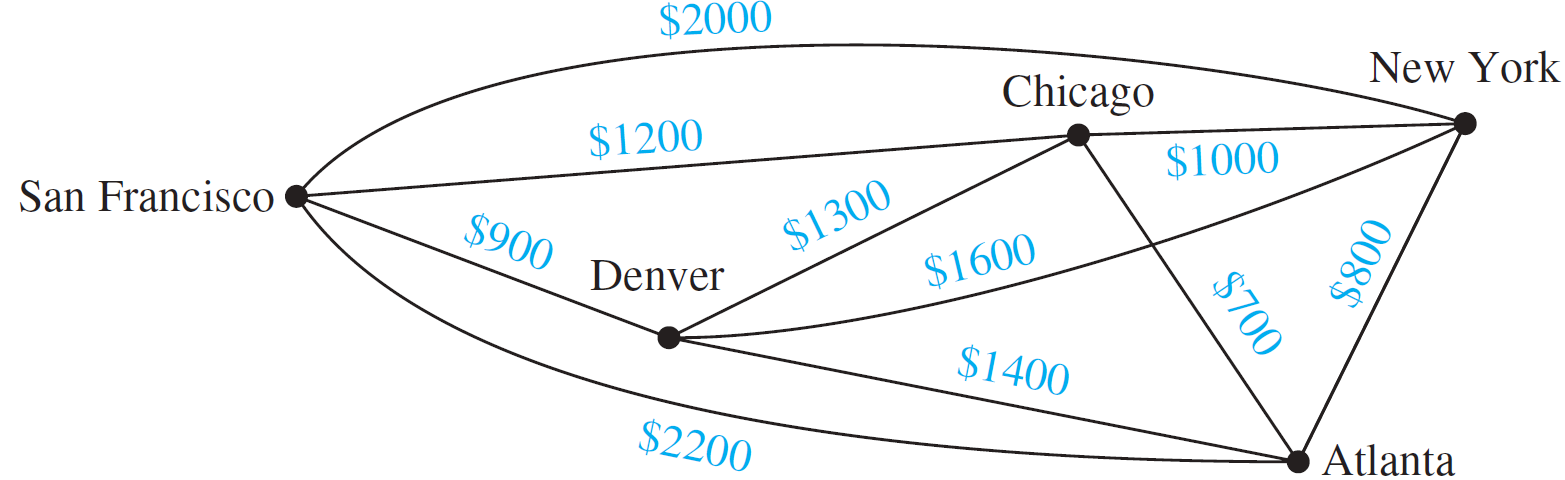
\includegraphics[width=.5\textwidth]{img/ch11.5-f1.png}
    \caption{A weighted graph showing monthly lease costs for lines in a computer network.}
    \label{fig:my_label}
\end{figure}

\subsection{Algorithms for Minimum Spanning Trees}

A wide variety of problems are solved by finding a spanning tree in a weighted graph such that the sum of the weights of the edges in the tree is a minimum.

\begin{definition}
{1}
A \textit{\textbf{minimum spanning tree}} in a connected weighted graph is a spanning tree that has the smallest possible sum of weights of its edges.
\end{definition}

There will be two algorithms for constructing minimum spanning trees. Both proceed by successively adding edges of smallest weight from those edges with a specified property that have not already been used. Both are greedy algorithms. Note that a greedy algorithm is a procedure that makes an optimal choice at each of its steps. Optimizing at each step does not guarantee that the optimal overall solution is produced. However, the two algorithms presented in this section for constructing minimum spanning trees are greedy algorithms that do produce optimal solutions.\\

The first algorithm is known as \textbf{Prim’s algorithm} (and sometimes as the \textbf{Prim-Jarník algorithm}). Begin by choosing any edge with smallest weight, putting it into the spanning tree. Successively add to the tree edges of minimum weight that are incident to a vertex already in the tree, never forming a simple circuit with those edges already in the tree. Stop when $n - 1$ edges have been added.

Later, it will be proved that this algorithm produces a minimum spanning tree for any connected weighted graph. Algorithm 1 gives a pseudocode description of Prim’s algorithm.

\begin{algorithm}
\caption{Prim’s Algorithm}
\begin{algorithmic}
\Procedure{$Prim$}{$G$: weighted connected undirected graph with $n$ vertices}
\State $T$ := a minimum-weight edge
\For{$i$ := $1$ to $n - 2$}
\State $e$ := an edge of minimum weight incident to a vertex in $T$ and not forming a simple circuit in $T$ if added to $T$
\State $T$ := $T$ with $e$ added
\EndFor
\State \Return{$T$} \{$T$ is a minimum spanning tree of $G$\}
\EndProcedure
\end{algorithmic}
\end{algorithm}

Note that the choice of an edge to add at a stage of the algorithm is not determined when there is more than one edge with the same weight that satisfies the appropriate criteria. We need to order the edges to make the choices deterministic. We will not worry about this in the remainder of the section. Also note that there may be more than one minimum spanning tree for a given connected weighted simple graph.

\begin{figure}[h!]
\begin{minipage}[c]{0.50\textwidth}
    \centering
    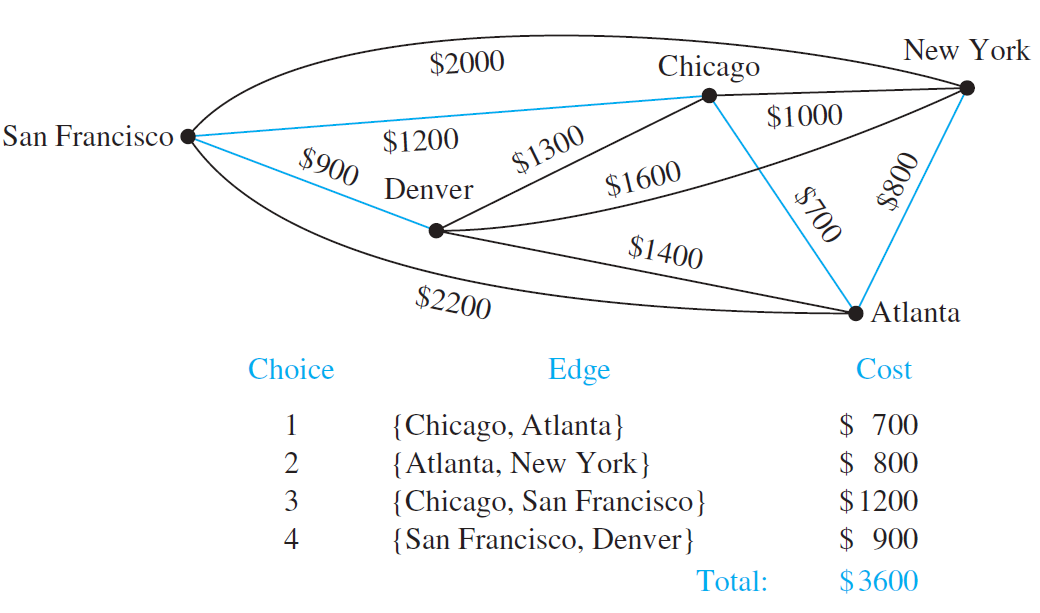
\includegraphics[width=\textwidth]{img/ch11.5-f2.png}
    \caption{A minimum spanning tree for the weighted graph in Figure 1.}
\end{minipage}\hfill
\begin{minipage}[c]{0.40\textwidth}
    \centering
    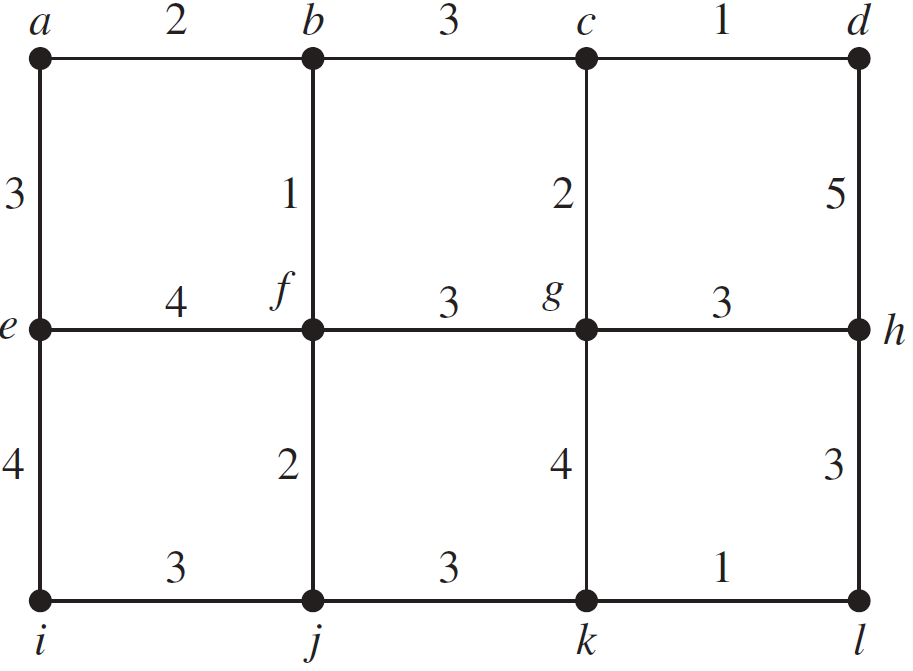
\includegraphics[width=\textwidth]{img/ch11.5-f3.png}
    \caption{A weighted graph}
\end{minipage}\hfill
\end{figure}

\begin{example}
Use Prim’s algorithm to design a minimum-cost communications network connecting all the computers represented by the graph in Figure 1.

\textbf{Solution:}
We solve this problem by finding a minimum spanning tree in the graph in Figure 1. Prim’s algorithm is carried out by choosing an initial edge of minimum weight and successively adding edges of minimum weight that are incident to a vertex in the tree and that do not form simple circuits. The edges in color in Figure 2 show a minimum spanning tree produced by Prim’s algorithm, with the choice made at each step displayed.
\end{example}

%\begin{figure}[h!]
%    \centering
%    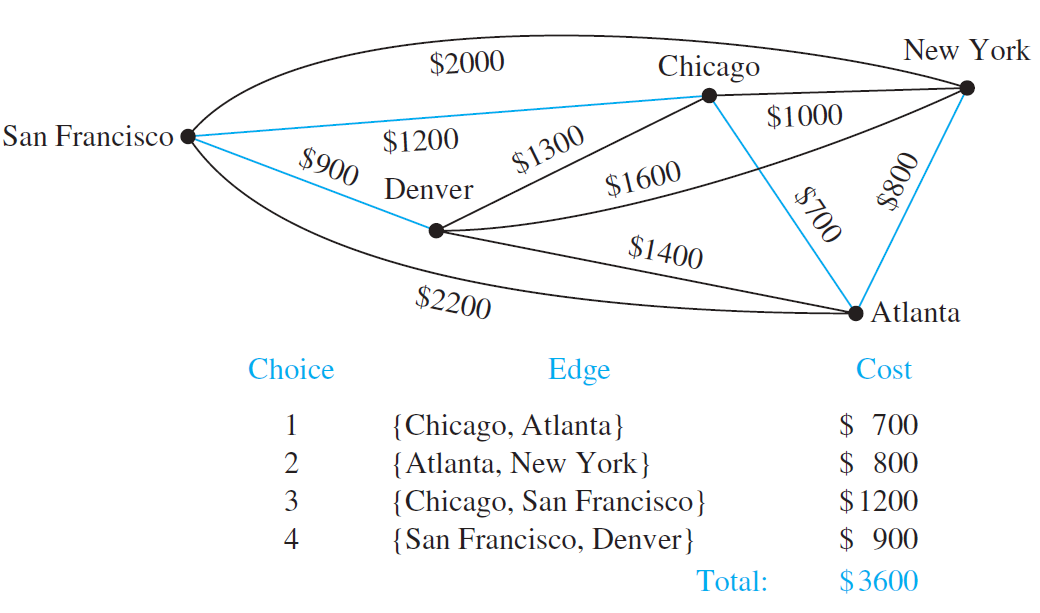
\includegraphics[width=\textwidth]{img/ch11.5-f2.png}
%    \caption{A minimum spanning tree for the weighted graph in Figure 1.}
%    \label{fig:my_label}
%\end{figure}

The second algorithm is \textbf{Kruskal’s algorithm}. To carry out Kruskal’s algorithm, choose an edge in the graph with minimum weight.

Successively add edges with minimum weight that do not form a simple circuit with those edges already chosen. Stop after $n - 1$ edges have been selected. Pseudocode for Kruskal’s algorithm is given in Algorithm 2.

\begin{algorithm}[h!]
\caption{Kruskal’s Algorithm}
\begin{algorithmic}
\Procedure{$Kruskal$}{$G$: weighted connected undirected graph with $n$ vertices}
\State $T$ := empty graph
\For{$i$ := $1$ to $n - 1$}
\State $e$ := any edge in $G$ with smallest weight that does not form a simple circuit when added to $T$
\State $T$ := $T$ with $e$ added
\EndFor
\State \Return{$T$} \{$T$ is a minimum spanning tree of $G$\}
\EndProcedure
\end{algorithmic}
\end{algorithm}

There is a difference between Prim’s and Kruskal’s algorithms. In Prim’s algorithm edges of minimum weight that are incident to a vertex already in the tree, and not forming a circuit, are chosen; whereas in Kruskal’s algorithm edges of minimum weight that are not necessarily incident to a vertex already in the tree, and that do not form a circuit, are chosen. 

Note that as in Prim’s algorithm, if the edges are not ordered, there may be more than one choice for the edge to add at a stage of this procedure. Consequently, the edges need to be ordered for the procedure to be deterministic.

\begin{example}
Use Kruskal’s algorithm to find a minimum spanning tree in the weighted graph shown in Figure 3.

\textbf{Solution:}
A minimum spanning tree and the choices of edges at each stage of Kruskal’s algorithm are shown in Figure 4.
\end{example}

\begin{figure}[h!]
    \centering
    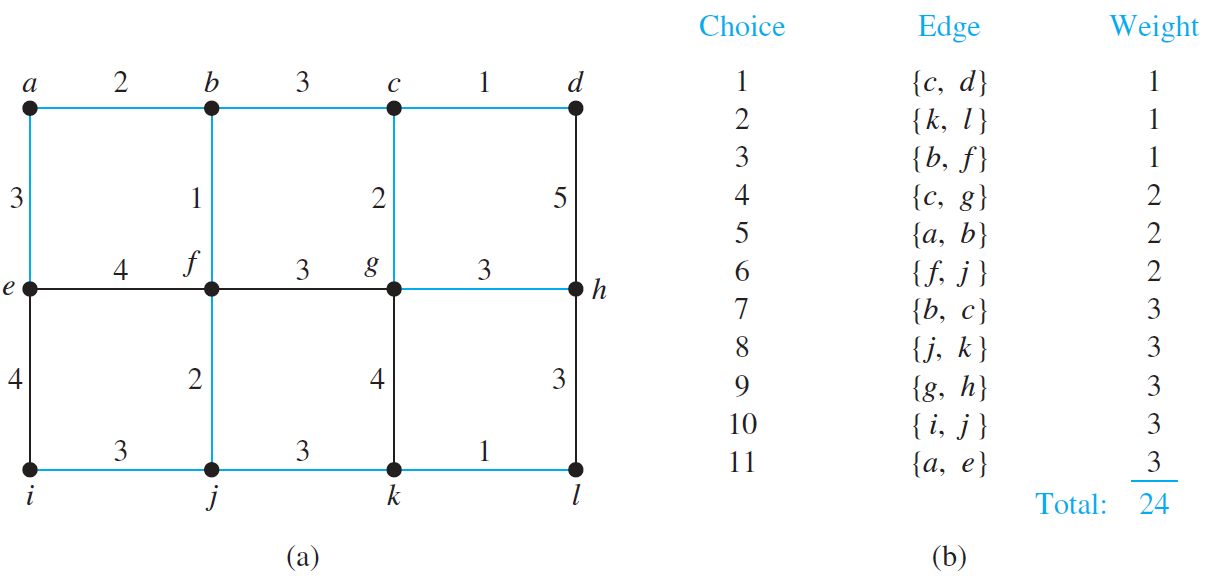
\includegraphics[width=.75\textwidth]{img/ch11.5-f5.png}
    \caption{A minimum spanning tree produced by Kruskal’s algorithm.}
    \label{fig:my_label}
\end{figure}

\textit{(The proof of the fact that Prim’s algorithm produces a minimum spanning tree of a connected weighted graph may be and should be read from textbook in page 838)}.

%\section*{Key Terms and Results}
%\textit{The following pages are retrieved directly from the textbook, pages 841 and 842}.

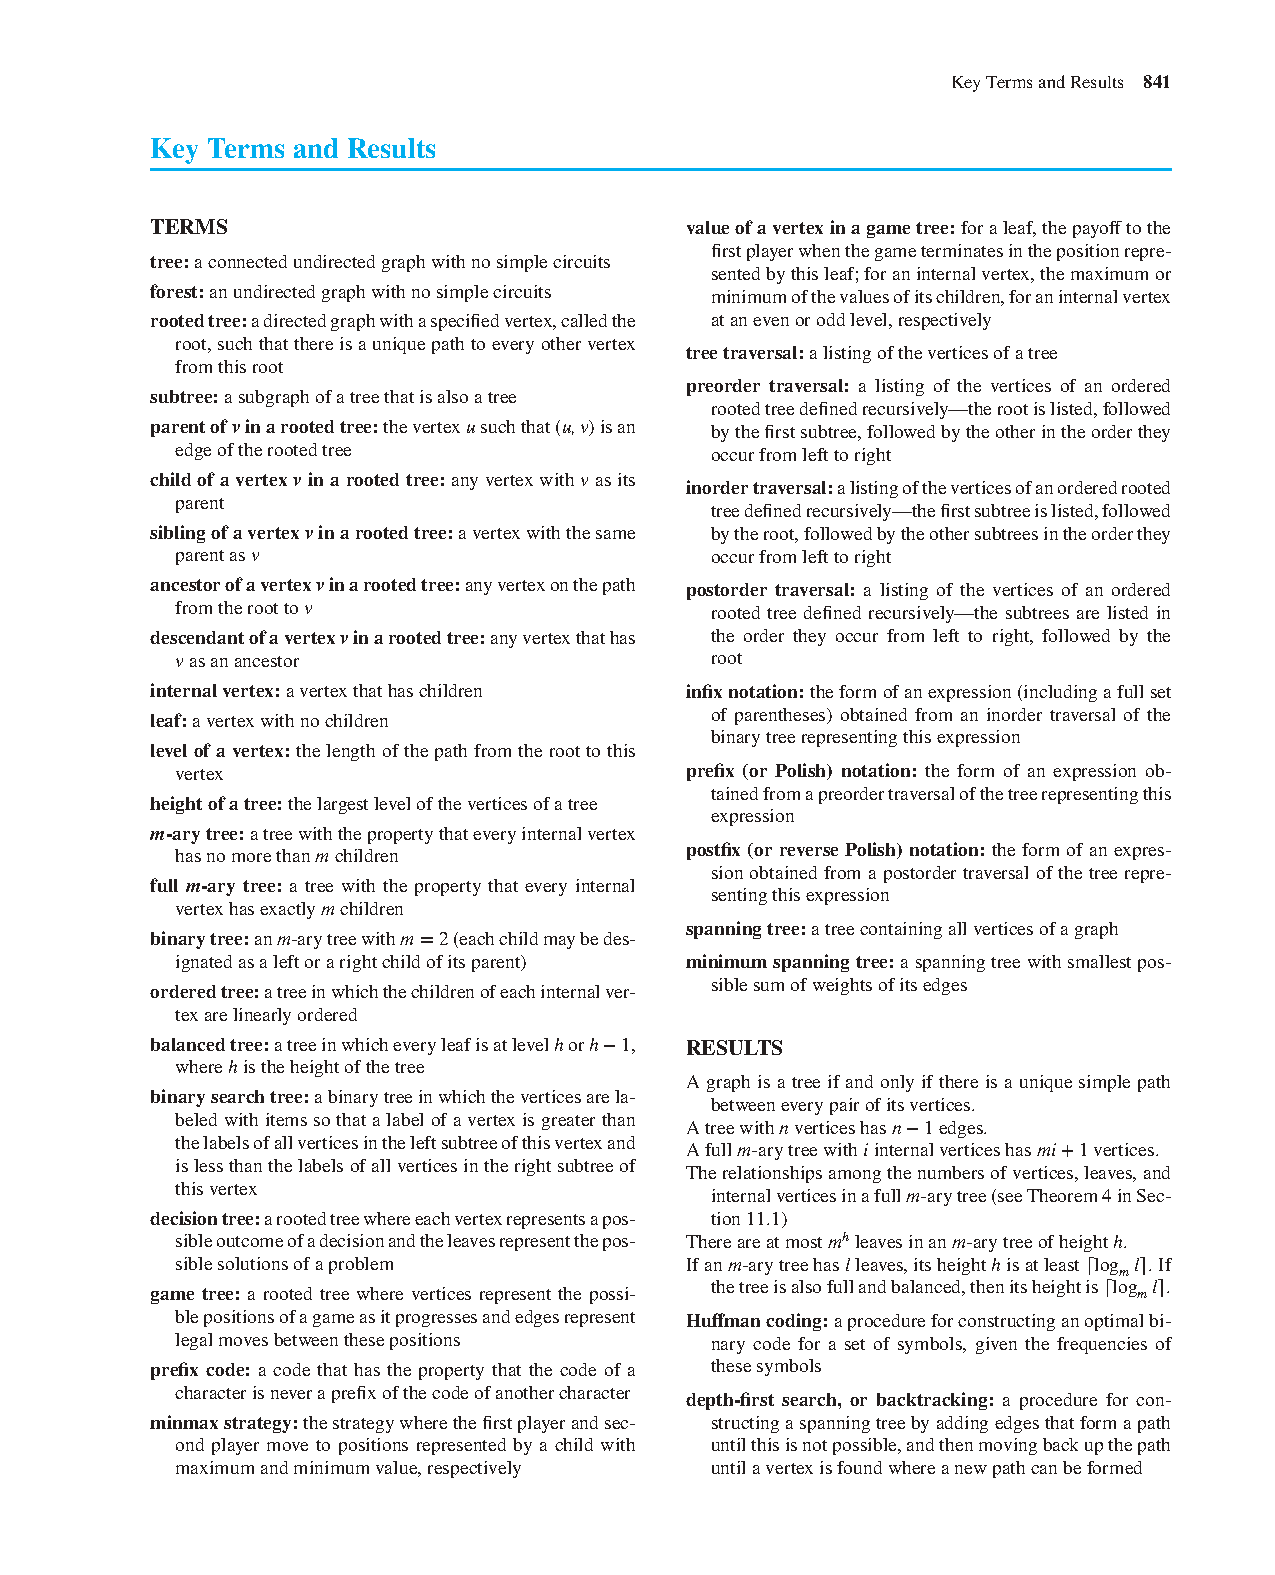
\includepdf[pages=1]{textbook-864_865}
\includepdf[pages=2]{textbook-864_865}


\end{document}
